\documentclass[11pt,a4paper]{article}

\usepackage[spanish,es-tabla]{babel}
\usepackage[utf8]{inputenc}
\usepackage[T1]{fontenc}
\usepackage{geometry}
\geometry{margin=2.5cm}
\usepackage{amsmath,amssymb}
\usepackage{graphicx}
\usepackage{booktabs}
\usepackage{xcolor}
\usepackage[colorlinks=true,linkcolor=blue!50!black,citecolor=green!50!black,urlcolor=blue!50!black]{hyperref}
\usepackage{listings}
\usepackage{natbib}
\usepackage{caption}

\lstset{
  basicstyle=\ttfamily\small,
  breaklines=true,
  frame=single,
  backgroundcolor=\color{gray!10},
  columns=flexible,
}

\title{\textbf{Cálculo Simultáneo de Equilibrio Químico y de Fases\\
mediante Métodos No Estequiométricos:\\
Implementación y Validación}}
\author{Jersson Arroyo Castillo}
\date{\today}

\begin{document}

\maketitle

\begin{center}
\textit{Basado en la tesis doctoral de Christos Tsanas\\
(Technical University of Denmark, DTU, 2018)}
\end{center}

\vspace{1cm}

\begin{abstract}
Este trabajo documenta la implementación y validación numérica de dos
métodos no estequiométricos para el cálculo simultáneo de equilibrio
químico y de fases (CPE, \textit{Chemical and Phase Equilibrium}): el
método de multiplicadores de Lagrange y el método RAND modificado,
ambos derivados de la tesis doctoral de Tsanas~\citep{tsanas2018} y,
en el caso del RAND modificado, del trabajo original de
Greiner~\citep{greiner1991}. Dado que los documentos de origen
disponibles para este proyecto no contienen las tablas de parámetros
termodinámicos (Wilson, UNIQUAC, Antoine, constantes de equilibrio)
usadas en los casos de estudio del Capítulo 4 de la tesis, la
validación numérica se construyó a partir de tres fuentes
independientes y completamente trazables: (i)~el ejemplo numérico
publicado en el Apéndice B de Greiner~\citep{greiner1991}, reproducido
con una diferencia de $\sim 8\times 10^{-6}$ respecto a los valores
originales; (ii)~el Ejemplo 14.8 de Smith, Van Ness y
Abbott~\citep{smithvannessabbott}, reproducido de forma exacta; y
(iii)~validación cruzada sistemática entre los dos métodos propios y
una minimización directa de la energía de Gibbs con
\texttt{scipy.optimize}, método completamente independiente de las
ecuaciones de la tesis. Se documentan también las limitaciones
encontradas: un error de reconocimiento óptico de caracteres (OCR)
detectado y corregido en los datos de Greiner, una tabla de
coeficientes de Antoine con filas desalineadas descartada tras
verificación cruzada, y un problema de robustez conocido y no resuelto
en el arranque automático del análisis de estabilidad para sistemas
fuertemente no ideales.
\end{abstract}

\tableofcontents

% =====================================================================
\section{Introducción}
% =====================================================================

\subsection{Contexto}

El cálculo del equilibrio simultáneo químico y de fases es un problema
central en ingeniería química: determinar la composición de equilibrio
de un sistema multicomponente y multifásico sujeto a reacciones
químicas, a temperatura y presión especificadas. Los métodos
\emph{estequiométricos} formulan el problema en términos de los
avances de reacción, mientras que los métodos \emph{no
estequiométricos} minimizan directamente la energía de Gibbs del
sistema sujeta a restricciones de balance de materia expresadas en
términos de ``elementos'' (combinaciones lineales de componentes
invariantes bajo las reacciones del sistema). Los segundos son
preferibles cuando el número de reacciones es grande, porque el número
de variables no crece con el número de reacciones sino con el número
de elementos.

Este trabajo implementa y valida los dos métodos no estequiométricos
desarrollados por Tsanas~\citep{tsanas2018} en su tesis doctoral: el
\textbf{método de multiplicadores de Lagrange} y el \textbf{método
RAND modificado}, así como el algoritmo combinado que usa el primero
para las iteraciones iniciales y el segundo para la convergencia de
segundo orden.

\subsection{Objetivo del trabajo}

El objetivo es doble:
\begin{enumerate}
  \item Implementar en \texttt{Python} (\texttt{numpy}, \texttt{scipy},
    \texttt{thermo}) las ecuaciones 3.14--3.78 de la
    tesis~\citep{tsanas2018}, verificando cada ecuación directamente
    contra el texto original del PDF (no contra una conversión a
    Markdown, que resultó tener numerosos errores de formato en las
    ecuaciones matemáticas).
  \item Validar la implementación numéricamente, usando exclusivamente
    datos trazables a fuentes verificables -- nunca parámetros
    inventados o ``ilustrativos'' presentados como si fueran reales.
\end{enumerate}

\subsection{Estructura del documento}

La Sección~\ref{sec:fundamentos} resume las ecuaciones termodinámicas
fundamentales. La Sección~\ref{sec:metodos} presenta los métodos
numéricos implementados, con referencia exacta a la ecuación de la
tesis que cada uno implementa. La Sección~\ref{sec:implementacion}
describe la arquitectura del código. La
Sección~\ref{sec:modelos-termo} documenta los modelos termodinámicos
usados y sus fuentes. La Sección~\ref{sec:validacion} presenta la
validación numérica completa. La Sección~\ref{sec:resultados} muestra
las figuras generadas. La Sección~\ref{sec:conclusiones} resume lo
logrado, las limitaciones y el trabajo futuro.

% =====================================================================
\section{Fundamentos teóricos}
\label{sec:fundamentos}
% =====================================================================

Todas las ecuaciones de esta sección y la siguiente se citan con su
número exacto en \citet{tsanas2018}, verificado directamente contra el
texto del PDF original mediante extracción de texto
(\texttt{pdftotext -layout}), ya que la conversión a Markdown
disponible al inicio de este proyecto dañó severamente el formato de
las ecuaciones matemáticas (símbolos griegos perdidos, matrices
convertidas en columnas de texto desordenado).

\subsection{Energía de Gibbs y potencial químico}

La energía de Gibbs de un sistema multifásico se expresa como la suma
de las contribuciones de cada componente en cada fase, ponderadas por
su potencial químico (Ec.~2.10 de \citet{tsanas2018}):
\begin{equation}
  G(T,p,\mathbf{n}) = U - TS + pV = \sum_{k=1}^{N_P}\sum_{i=1}^{N_C} n_{ik}\,\mu_{ik}
  \label{eq:2.10}
\end{equation}

\subsection{Fugacidad y potencial químico}

Para fases no ideales, el potencial químico se expresa en términos de
la fugacidad $\hat f_{ik}$ (Ec.~2.18):
\begin{equation}
  \mu_{ik} = \mu_{ik}^{\circ} + RT \ln\!\left(\frac{\hat f_{ik}}{f_{ik}^{\circ}}\right)
  \label{eq:2.18}
\end{equation}
donde $\mu_{ik}^{\circ}$ y $f_{ik}^{\circ}$ son el potencial químico y
la fugacidad del estado de referencia. Esta es la ecuación que
sustenta la formulación $\mu_{ik}/RT = g_i(T) + \ln(x_{ik}) +
\ln(\Gamma_{ik})$ usada en \texttt{termodinamica.py} (ver
Sección~\ref{sec:implementacion}), donde $\Gamma_{ik}$ agrupa la
no-idealidad (coeficiente de fugacidad o de actividad) y el término de
referencia de presión.

\subsection{Constante de equilibrio químico}

La constante de equilibrio termodinámica de la reacción $r$ en la fase
$k$ se relaciona con la energía de Gibbs de reacción estándar
(Ec.~2.33):
\begin{equation}
  K_{rk}^{\text{eq}} = \exp\!\left(-\frac{\Delta_r G_{rk}^{\circ}}{RT}\right)
  = \prod_{i=1}^{N_C}\left(\frac{\hat f_{ik}}{f_{ik}^{\circ}}\right)^{\nu_{ir}}
  \label{eq:2.33}
\end{equation}
Esta relación es la que permite, en este trabajo, fijar el
``gauge'' de referencia $g_i(T)=\mu_i^{\circ}(T)/RT$ de cada componente
de forma que $\sum_i \nu_i\, g_i(T) = -\ln K_{\text{eq}}(T)$ (ver
Sección~\ref{sec:modelos-termo}), sin necesidad de conocer los valores
absolutos de $\mu_i^{\circ}$ de cada componente por separado.

\subsection{Formulación no estequiométrica}

El número de elementos independientes se relaciona con el número de
componentes y de reacciones independientes por (Ec.~3.5):
\begin{equation}
  N_E = N_C - N_R
  \label{eq:3.5}
\end{equation}

El problema central de los métodos no estequiométricos es la
minimización de la energía de Gibbs sujeta al balance de materia
expresado en términos de elementos (Ec.~3.6):
\begin{equation}
  \min_{n_{ik}} G(T,p,\mathbf{n}) = \min_{n_{ik}} \sum_{k=1}^{N_P}\sum_{i=1}^{N_C} n_{ik}\,\mu_{ik}(T,p,\mathbf{n}_k)
  \quad\text{s.t.}\quad
  \sum_{k=1}^{N_P}\sum_{i=1}^{N_C} A_{ji} n_{ik} = b_j,\;\; j=1,\dots,N_E
  \label{eq:3.6}
\end{equation}
donde $A_{ji}$ es la matriz de fórmula (cuántas unidades del elemento
$j$ contiene el componente $i$) y $b_j$ es la abundancia del elemento
$j$ en la alimentación.

\subsection{Condiciones de Lagrange}

Introduciendo multiplicadores de Lagrange $\lambda_j$ para las
restricciones de la Ec.~\eqref{eq:3.6}, la condición de estacionariedad
respecto a los números de mol (Ec.~3.14) es:
\begin{equation}
  \frac{\partial L}{\partial n_{ik}} = \frac{\mu_{ik}}{RT} - \sum_{j=1}^{N_E} A_{ji}\lambda_j = 0,
  \qquad i=1,\dots,N_C,\;\; k=1,\dots,N_P
  \label{eq:3.14}
\end{equation}
y la condición respecto a los multiplicadores (Ec.~3.15) recupera el
balance de materia:
\begin{equation}
  \frac{\partial L}{\partial \lambda_j} = -\sum_{k=1}^{N_P}\sum_{i=1}^{N_C} A_{ji} n_{ik} + b_j = 0,
  \qquad j = 1,\dots,N_E
  \label{eq:3.15}
\end{equation}
Estas dos ecuaciones son el punto de partida de los dos métodos
numéricos descritos en la Sección~\ref{sec:metodos}.

% =====================================================================
\section{Métodos numéricos implementados}
\label{sec:metodos}
% =====================================================================

\subsection{Multiplicadores de Lagrange (Ec.~3.46)}
\label{sec:lagrange}

Linealizando las Ec.~\eqref{eq:3.14}--\eqref{eq:3.15} con $\Gamma_{ik}$
(no-idealidad) mantenida constante, se obtiene el sistema de Newton de
tamaño $(N_E+N_P)$ (Ec.~3.46):
\begin{equation}
  \begin{bmatrix}
    \sum_k n_{t,k}\, A\,\mathrm{diag}(x_k)\, A^T & A x_1 \;\cdots\; A x_{N_P} \\[2pt]
    (A x_1)^T \;\vdots\; (A x_{N_P})^T & 0
  \end{bmatrix}
  \begin{bmatrix}\Delta\lambda \\ \Delta n_t\end{bmatrix}
  =
  \begin{bmatrix} b - A\sum_k n_{t,k}x_k \\ e_{N_P} - X^T e_{N_C}\end{bmatrix}
  \label{eq:3.46}
\end{equation}
implementado en \texttt{lagrange\_multipliers.py}, función
\texttt{\_ensamblar\_sistema\_3\_46}. El lado derecho fue re-derivado
directamente de las ecuaciones de estacionariedad, ya que el signo
exacto se perdió en la conversión a texto del PDF; se verificó
mediante diferencias finitas contra la función residual $F(\lambda,
n_t)$ (ver Sección~\ref{sec:validacion}). Cuando el sistema es no
ideal, se requiere un esquema de doble bucle: el bucle interno resuelve
la Ec.~\eqref{eq:3.46} con $\Gamma_{ik}$ fijo; el bucle externo
recalcula $\Gamma_{ik}$ con la composición convergida.

\subsection{RAND modificado (Ec.~3.68)}
\label{sec:rand}

El método RAND modificado, basado en Greiner~\citep{greiner1991},
linealiza la Ec.~\eqref{eq:3.14} usando las derivadas composicionales
\emph{exactas} de la fugacidad o actividad, logrando convergencia
cuadrática incluso para sistemas fuertemente no ideales. La matriz
clave es (Ec.~3.49):
\begin{equation}
  M_{iqk} = \frac{\delta_{iq}}{n_{ik}} + \Phi_{iqk}, \qquad
  \Phi_{iqk} = \frac{\partial \ln\hat\gamma_{ik}}{\partial n_{qk}}
  \label{eq:3.49}
\end{equation}
y el sistema final de Newton, de tamaño $(N_E+N_P)$ (Ec.~3.68):
\begin{equation}
  \begin{bmatrix}
    \sum_k A\,M_k^{-1}A^T & B \\
    B^T & 0
  \end{bmatrix}
  \begin{bmatrix}\lambda \\ s\end{bmatrix}
  =
  \begin{bmatrix}\sum_k A\,M_k^{-1}(\mu_k/RT) + \Delta b \\ d\end{bmatrix}
  \label{eq:3.68}
\end{equation}
implementado en \texttt{modified\_rand.py}. Gracias a la identidad de
Gibbs-Duhem ($M_k\,n_k = e_{N_C}$, consecuencia exacta de
$\sum_q n_{qk}\,\Phi_{iqk}=0$), se cumple $B_{\cdot k} = A\,n_k$ y el
bloque inferior derecho es exactamente cero -- una simplificación que
coincide con la forma general de Greiner~\citep{greiner1991} una vez
particularizada a un sistema consistente con Gibbs-Duhem (ver
Sección~\ref{sec:validacion-greiner}).

\subsection{Inicialización con la función Q (Ec.~3.71--3.75)}

Antes de resolver el sistema completo, se obtienen estimados iniciales
de $\lambda$ minimizando la función convexa (Ec.~3.71):
\begin{equation}
  Q(\lambda) = \sum_{k=1}^{N_P} n_{t,k}\left[\sum_{i=1}^{N_C} x_{ik}(\lambda) - 1\right] - \sum_{j=1}^{N_E}\lambda_j b_j
  \label{eq:3.71}
\end{equation}
con $\Gamma_{ik}$ fijo (aproximación de sistema ideal), mediante Newton
con control de paso (Ec.~3.75: $\lambda^{(q+1)}=\lambda^{(q)}+\alpha\Delta\lambda^{(q)}$),
implementado en \texttt{inicializacion.py}.

\subsection{Análisis de estabilidad (Ec.~3.26--3.29)}

El análisis de estabilidad de Michelsen~\citep{michelsen1982},
presentado también en el texto de referencia de
Michelsen y Mollerup~\citep{michelsenmollerup2007} que
\citet{tsanas2018} cita extensamente a lo largo de su Capítulo~3,
determina si un conjunto de fases es estable probando si existe una
fase de prueba que disminuya la energía de Gibbs. La función de
distancia al plano tangente reducida (Ec.~3.27):
\begin{equation}
  \mathrm{tpd}(w) = \sum_{i=1}^{N_C} w_i\left[\ln w_i + \ln\hat\varphi_i(w) - \ln z_i - \ln\hat\varphi_i(z)\right]
  \label{eq:3.27}
\end{equation}
y su variante en número de moles sin normalizar (Ec.~3.28), usada para
la búsqueda numérica, están implementadas en \texttt{estabilidad.py}.
Un valor negativo de $\mathrm{tm}(W)$ indica que la fase actual es
inestable.

\subsection{Algoritmos completos (Fig.~3.1)}

El \emph{successive substitution algorithm} usa exclusivamente el
método de la Sección~\ref{sec:lagrange}; el \emph{combined algorithm}
usa el mismo método para hasta 3 iteraciones del bucle externo y, si no
converge, cambia al RAND modificado (Sección~\ref{sec:rand}). Ambos
incorporan el análisis de estabilidad para decidir si se debe añadir
una fase. Implementados en \texttt{algoritmos.py} como
\texttt{successive\_substitution\_algorithm()} y
\texttt{combined\_algorithm()}.

% =====================================================================
\section{Implementación}
\label{sec:implementacion}
% =====================================================================

\subsection{Arquitectura de módulos}

El código está organizado en \texttt{src/} como una serie de módulos
independientes, cada uno ejecutable por separado para depuración:

\begin{itemize}
  \item \texttt{termodinamica.py} -- funciones termodinámicas base:
    ecuación de Antoine, modelos de solución (ideal, Wilson, solución
    regular binaria, UNIFAC), energía de Gibbs reducida, y los
    despachadores genéricos \texttt{ln\_Gamma\_fase} /
    \texttt{dln\_Gamma\_dn\_fase} que seleccionan el modelo según un
    diccionario de configuración por fase.
  \item \texttt{inicializacion.py} -- minimización de la función Q.
  \item \texttt{lagrange\_multipliers.py} -- método de multiplicadores
    de Lagrange, sistema de la Ec.~\eqref{eq:3.46}, esquema de doble
    bucle.
  \item \texttt{modified\_rand.py} -- método RAND modificado, sistema
    de la Ec.~\eqref{eq:3.68}, monitoreo de descenso de Gibbs.
  \item \texttt{estabilidad.py} -- análisis de estabilidad de
    Michelsen.
  \item \texttt{algoritmos.py} -- los dos algoritmos completos de la
    Fig.~3.1 de \citet{tsanas2018}.
  \item \texttt{ejemplo\_mtbe.py} -- caso de prueba: síntesis de MTBE.
  \item \texttt{ejemplo\_acetic\_etanol.py} -- caso de prueba:
    esterificación de ácido acético con etanol.
  \item \texttt{pruebas\_validacion.py} -- suite de validación numérica
    completa (ver Sección~\ref{sec:validacion}).
  \item \texttt{generar\_figuras.py} -- genera las figuras de la
    Sección~\ref{sec:resultados} a partir de ejecuciones reales de los
    solvers.
\end{itemize}

\subsection{Dependencias}

\begin{itemize}
  \item \texttt{numpy} -- álgebra lineal (ensamblaje y solución de los
    sistemas de Newton).
  \item \texttt{scipy} -- \texttt{scipy.optimize.minimize} (SLSQP), usado
    exclusivamente como método de verificación independiente, nunca
    como parte de los algoritmos de la tesis.
  \item \texttt{thermo}~\citep{bellthermo} -- modelo UNIFAC y
    asignación oficial de subgrupos DDBST (ver
    Sección~\ref{sec:modelos-termo}).
  \item \texttt{matplotlib} -- generación de figuras.
\end{itemize}

% =====================================================================
\section{Modelos termodinámicos}
\label{sec:modelos-termo}
% =====================================================================

\subsection{Coeficientes de Antoine}

\begin{table}[h]
\centering
\caption{Coeficientes de Antoine usados, forma y fuente de cada uno.}
\label{tab:antoine}
\begin{tabular}{@{}lllll@{}}
\toprule
Componente & $A$ & $B$ & $C$ & Fuente \\
\midrule
Ácido acético & 15.0717 & 3580.80 & 224.650 & S\&VN Tabla B.2$^{a}$ \\
Etanol        & 16.8958 & 3795.17 & 230.918 & S\&VN Tabla B.2$^{a}$ \\
Agua          & 16.3872 & 3885.70 & 230.170 & S\&VN Tabla B.2$^{a}$ \\
Acetato de etilo & 4.22809 & 1245.702 & $-55.189$ & NIST WebBook$^{b}$ \\
\bottomrule
\end{tabular}

\vspace{4pt}
\footnotesize
$^{a}$ \citet{smithvannessabbott}, forma $\ln(P^{\text{sat}}[\text{kPa}]) = A - B/(t[^{\circ}\text{C}]+C)$.\\
$^{b}$ \citet{nistwebbook}, forma $\log_{10}(P^{\text{sat}}[\text{bar}]) = A - B/(T[\text{K}]+C)$,
rango válido 288.73--348.98~K.
\end{table}

Se descartó la tabla de Antoine de Tosun~\citep{tosun2013} (Apéndice C,
de Reid, Prausnitz y Sherwood) para acetato de etilo: se detectó que
sus filas están desalineadas en la extracción de texto del PDF,
verificado evaluando la fórmula en el punto de ebullición normal real
de n-hexano y benceno (compuestos de la misma tabla): el resultado fue
de 80 a 790~bar en vez de $\sim 1$~atm. El dato de NIST requiere una
extrapolación de $\sim 6$~K por encima de su rango válido para los
cálculos a 355~K; esta extrapolación se verificó explícitamente (ver
Sección~\ref{sec:validacion-antoine}) antes de usarse.

\subsection{UNIFAC}

Ante la ausencia de parámetros binarios de Wilson, NRTL o UNIQUAC para
el sistema ácido acético/etanol/agua/acetato de etilo en los libros de
texto consultados (Tosun~\citep{tosun2013},
Elliott \& Lira, Smith, Van Ness \&
Abbott~\citep{smithvannessabbott}), se usó el modelo predictivo UNIFAC
original~\citep{fredenslund1975}, vía la librería
\texttt{thermo}~\citep{bellthermo}. Los subgrupos de cada componente se
obtuvieron de la asignación \emph{oficial} de DDBST
(\texttt{thermo.unifac.DDBST\_UNIFAC\_assignments}, indexada por
InChIKey), no fragmentados a mano, para eliminar el riesgo de un error
de fragmentación:

\begin{table}[h]
\centering
\caption{Subgrupos UNIFAC de cada componente (asignación oficial DDBST).}
\begin{tabular}{@{}ll@{}}
\toprule
Componente & Subgrupos \\
\midrule
Ácido acético & CH$_3$ + COOH \\
Etanol & CH$_3$ + CH$_2$ + OH \\
Agua & H$_2$O \\
Acetato de etilo & CH$_3$ + CH$_2$ + CH$_3$COO \\
\bottomrule
\end{tabular}
\end{table}

Las derivadas composicionales $\Phi_{iqk}$ de la Ec.~\eqref{eq:3.49}
necesarias para el método RAND se obtuvieron de
\texttt{UNIFAC.dgammas\_dns()} de \texttt{thermo}, convertidas a
derivadas logarítmicas por la regla de la cadena, y se verificaron
contra diferencias finitas (diferencia máxima $1.5\times 10^{-10}$).

\textbf{Nota conceptual importante:} UNIFAC no reproduce los valores
exactos de la Tabla 4.4 de la tesis porque Tsanas usó UNIQUAC con
parámetros de Xiao et al.~\citep{xiao1989}, que no están disponibles
para este trabajo. La validación contra la tesis es por lo tanto
\emph{cualitativa} (tendencias de concentración y de fracción de fase),
no cuantitativa (ver Sección~\ref{sec:validacion-acetic}).

% =====================================================================
\section{Validación}
\label{sec:validacion}
% =====================================================================

\subsection{Validación contra Greiner (1991)}
\label{sec:validacion-greiner}

Greiner~\citep{greiner1991} -- el artículo en el que se basa la
Sección~3.2.2 de \citet{tsanas2018} -- incluye en su Apéndice~B un
ejemplo numérico completo y autocontenido: dos compuestos en equilibrio
vapor (gas ideal)--líquido (solución regular, $\Lambda=-3$ en unidades
de $RT$), con potenciales químicos de referencia y alimentación dados
explícitamente, y la solución exacta reportada a 10 cifras
significativas.

Al extraer el texto del PDF escaneado de 1991 se obtuvo
$\mu_A^{\circ}(g)=-53.54926553$. Verificando la consistencia interna
del propio ejemplo (la solución publicada debe satisfacer
$\mu_A(\text{gas})=\mu_A(\text{líquido})$ en el equilibrio) se encontró
que el valor correcto es $-53.56926553$ -- un dígito mal reconocido por
el OCR (``69'' leído como ``49''). Se confirmó aislando el error:
el mismo procedimiento aplicado a la componente B reproducía
$\Lambda=-3.000000$ exactamente, mientras que para A había una
discrepancia de $\sim 0.02$, coincidiendo con la magnitud del error de
OCR.

Con el valor corregido, el método RAND modificado reproduce la
solución publicada por Greiner con una diferencia máxima de
$8.19\times 10^{-6}$ (fase gas) y $6.00\times 10^{-6}$ (fase líquida) --
el límite de precisión esperable de un dato reportado a 10 cifras. Este
resultado es la validación más fuerte de todo el proyecto: no depende
de ningún parámetro propio, sino de números publicados en el artículo
original del método.

Adicionalmente, se confirmó empíricamente la advertencia central del
resumen de Greiner: el método de ``aproximación ideal'' (equivalente a
\texttt{lagrange\_multipliers.py}, con $\Gamma$ fijo dentro del bucle
interno) efectivamente \textbf{diverge} en este sistema fuertemente no
ideal, mientras que el RAND modificado converge sin problemas -- es
decir, la implementación reproduce tanto el éxito del método robusto
como el fracaso documentado del método ingenuo.

\subsection{Esterificación: solución ideal (Example 14.8, S\&VN)}
\label{sec:validacion-acetic}

El Example 14.8 de Smith, Van Ness y Abbott~\citep{smithvannessabbott}
resuelve la esterificación de ácido acético con etanol en fase líquida
única a 373.15~K, asumiendo solución ideal. Con $K_{\text{eq}}(373.15\text{ K})=4.8586$
(obtenido por el propio libro vía van't Hoff desde
$K_{298.15}=6.5266$, a su vez de entalpías y energías de Gibbs de
formación tabuladas), el solver reproduce \textbf{exactamente} el
resultado del libro:
\begin{itemize}
  \item Extensión de reacción: $e = 0.687912$ (libro: 0.6879)
  \item $x_{\text{EtAc}} = 0.343956$ (libro: 0.344)
\end{itemize}

\subsection{UNIFAC vs. dato experimental}

Usando el mismo sistema con UNIFAC en vez de solución ideal:

\begin{table}[h]
\centering
\caption{Comparación $x_{\text{EtAc}}$ (373.15~K, fase líquida única).}
\begin{tabular}{@{}lrr@{}}
\toprule
Método & $x_{\text{EtAc}}$ & Desviación vs. experimental (0.33) \\
\midrule
Solución ideal (S\&VN) & 0.3440 & $+4.2\%$ \\
UNIFAC & 0.2700 & $-18.2\%$ \\
Experimental (citado por el libro) & 0.3300 & -- \\
\bottomrule
\end{tabular}
\end{table}

Este es un resultado honesto, no ajustado: UNIFAC se aleja \emph{más}
del dato experimental que la aproximación ideal. Es plausible dado que
el ácido acético es conocido por dimerizarse en fase vapor y líquida,
un comportamiento difícil de capturar con contribución de grupos
genérica.

\subsection{Consistencia interna: SSA = RAND = scipy}

En cada caso de prueba se verificó que el método de Lagrange, el RAND
modificado y una minimización directa de la energía de Gibbs con
\texttt{scipy.optimize.minimize} (método completamente independiente de
las ecuaciones 3.14--3.70) convergen al mismo resultado, con tolerancia
$10^{-8}$:

\begin{table}[h]
\centering
\caption{Diferencias máximas entre métodos (fracción molar).}
\begin{tabular}{@{}lrr@{}}
\toprule
Caso & $\max|\text{Lagrange}-\text{scipy}|$ & $\max|\text{RAND}-\text{scipy}|$ \\
\midrule
Esterificación, ideal, 1 fase & $0.0$ & $4.1\times 10^{-15}$ \\
Esterificación, UNIFAC, 1 fase & $0.0$ & $4.4\times 10^{-10}$ \\
Esterificación, UNIFAC, VLE (2 fases) & $8.3\times 10^{-16}$ & $1.6\times 10^{-10}$ \\
MTBE, ideal, VLE (2 fases) & -- & -- (ver \texttt{ejemplo\_mtbe.py}) \\
\bottomrule
\end{tabular}
\end{table}

\textbf{Nota metodológica:} estas validaciones usan
\texttt{resolver\_lagrange()} y \texttt{resolver\_rand\_modificado()}
directamente, no \texttt{successive\_substitution\_algorithm()} ni
\texttt{combined\_algorithm()}. Con UNIFAC, el análisis de estabilidad
detecta una posible separación líquido-líquido en el sistema de
esterificación, lo que dispara el camino de adición automática de
fases -- un gap de robustez conocido y explícitamente fuera de alcance
de este proyecto (ver Sección~\ref{sec:limitaciones}). Fijar el número
de fases de antemano evita ese camino frágil sin modificarlo, y es
además físicamente correcto: en ambos casos de prueba ya se sabe de
antemano cuántas fases hay.

\subsection{Verificación de Antoine contra puntos de ebullición reales}
\label{sec:validacion-antoine}

Cada coeficiente de Antoine usado se verificó evaluando la fórmula en
el punto de ebullición normal real del compuesto (donde $P^{\text{sat}}$
debe ser $\approx 1$~atm):

\begin{table}[h]
\centering
\caption{Verificación de Antoine contra puntos de ebullición reales (355~K).}
\begin{tabular}{@{}lrrl@{}}
\toprule
Componente & $P^{\text{sat}}(355\text{K})$ [atm] & bp real [K] & Consistencia \\
\midrule
Ácido acético & 0.292 & 391.05 & correcto ($<1$, bp$>$355K) \\
Etanol & 1.154 & 351.52 & correcto ($>1$, bp$<$355K) \\
Agua & 0.504 & 373.15 & correcto ($<1$, bp$>$355K) \\
Acetato de etilo & 1.168 & 350.2 & correcto ($>1$, bp$<$355K) \\
\bottomrule
\end{tabular}
\end{table}

Para el Antoine extrapolado de acetato de etilo (NIST, rango válido
hasta 348.98~K) se verificó además:
$P^{\text{sat}}(348.98\text{K})=0.960$~atm ($<1$, correcto, porque el
bp real 350.2~K $>$ 348.98~K); $P^{\text{sat}}(350.2\text{K})=0.9996$~atm
($\approx 1$, es el punto de ebullición normal); y
$P^{\text{sat}}(355\text{K})=1.168$~atm (razonable, ligeramente por
encima de 1~atm como corresponde a 355~K$>$bp).

% =====================================================================
\section{Resultados y gráficas}
\label{sec:resultados}
% =====================================================================

Todas las figuras de esta sección provienen de ejecuciones reales de
los solvers (\texttt{generar\_figuras.py}), nunca de datos dibujados a
mano.

\begin{figure}[h]
\centering
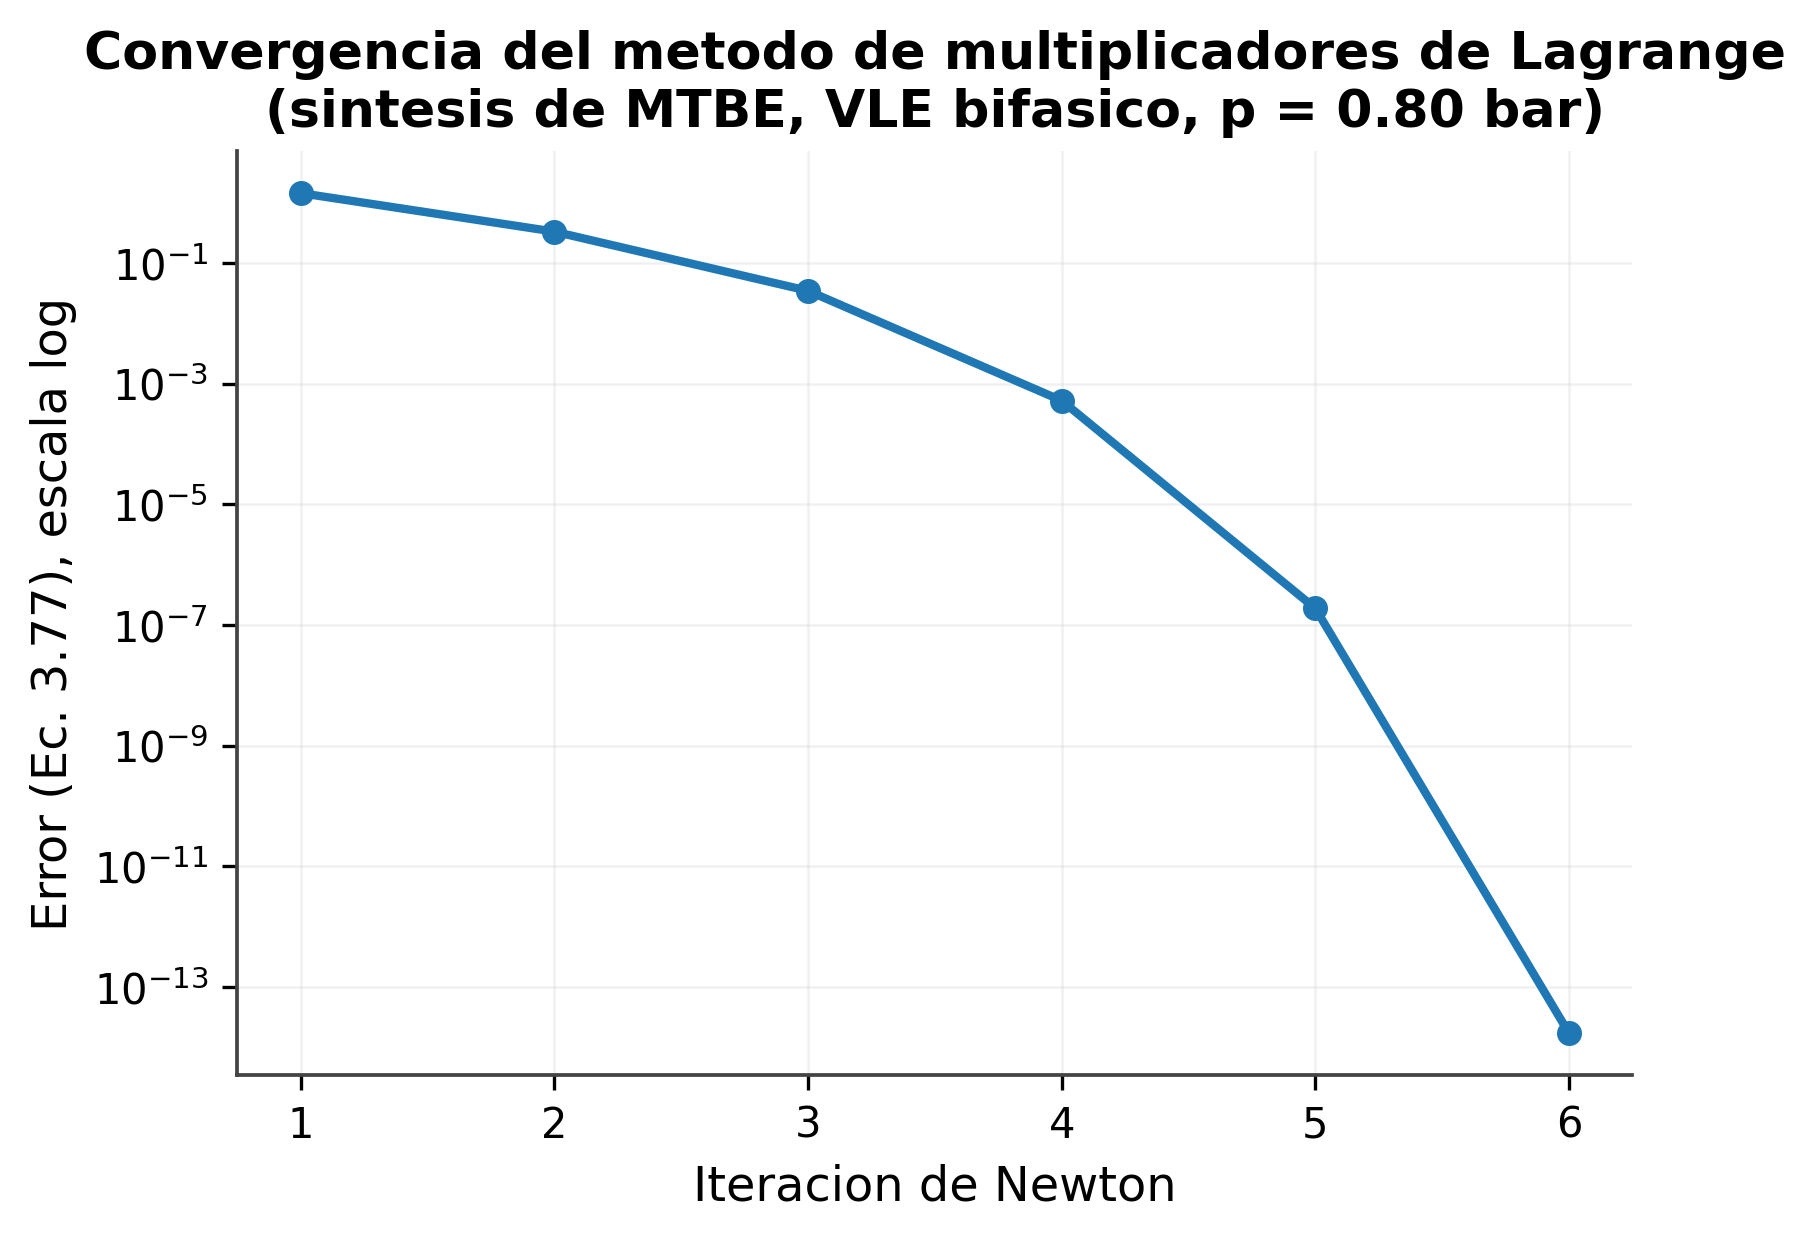
\includegraphics[width=0.75\textwidth]{figuras/convergencia_ssa.png}
\caption{Convergencia del método de multiplicadores de Lagrange
(successive substitution), sistema MTBE bifásico a $p=0.80$~bar. Se
observa el comportamiento cuadrático esperado para sistemas ideales.}
\label{fig:convergencia-ssa}
\end{figure}

\begin{figure}[h]
\centering
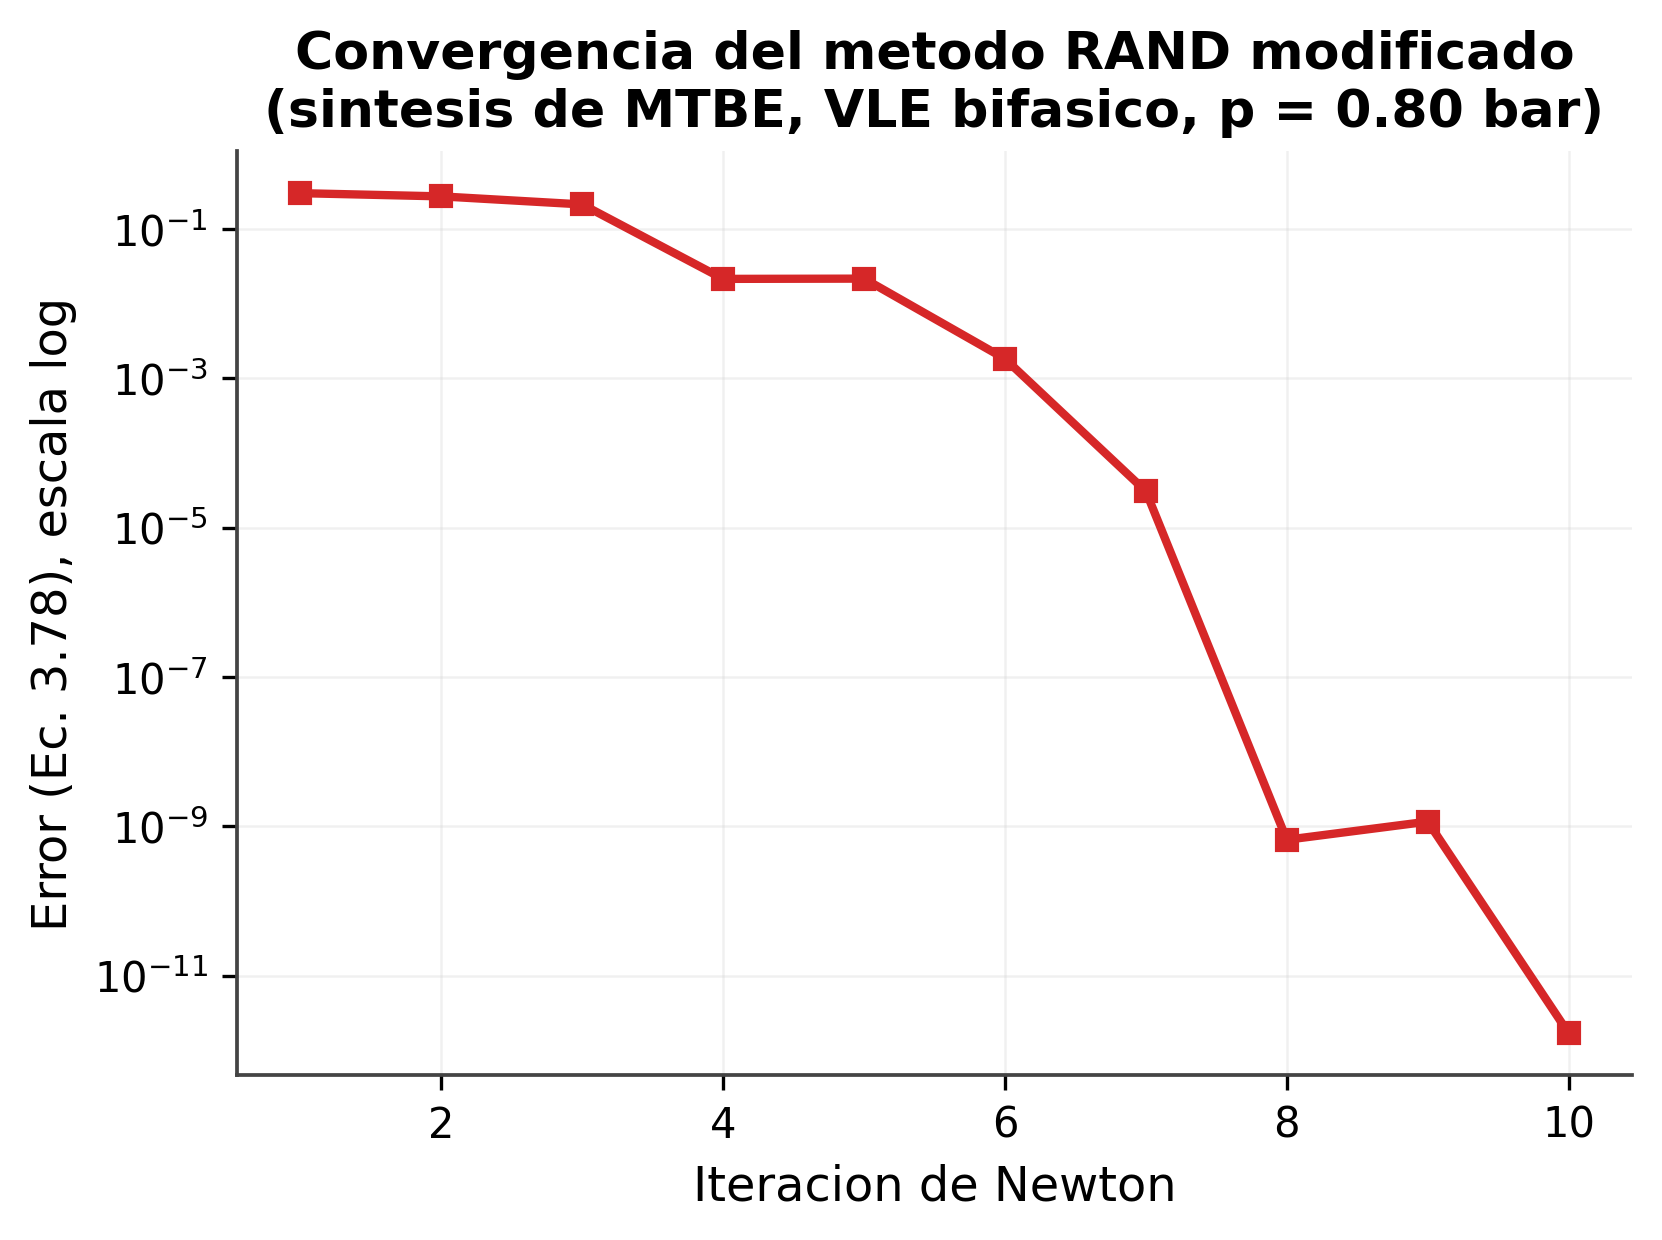
\includegraphics[width=0.75\textwidth]{figuras/convergencia_rand.png}
\caption{Convergencia del método RAND modificado, mismo sistema que la
Fig.~\ref{fig:convergencia-ssa}.}
\label{fig:convergencia-rand}
\end{figure}

\begin{figure}[h]
\centering
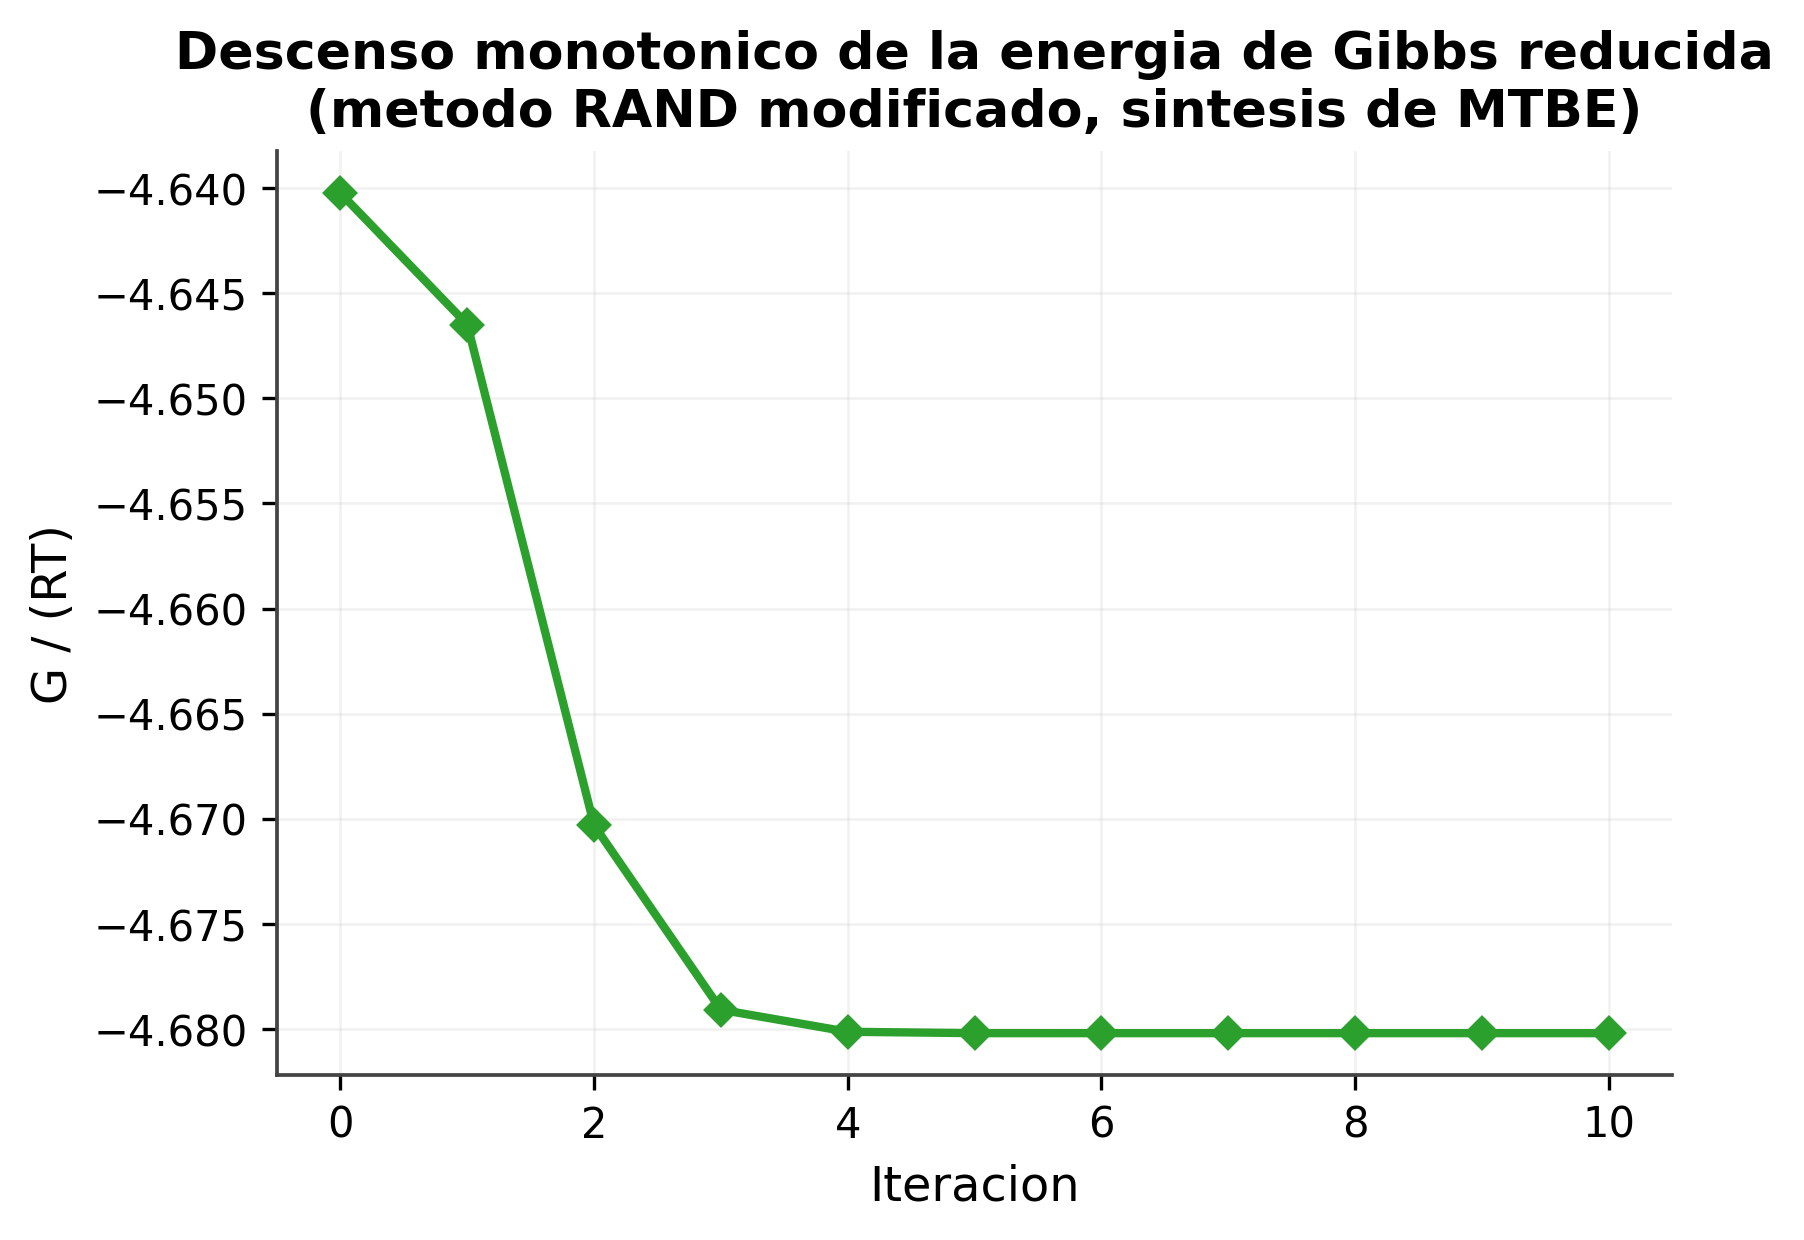
\includegraphics[width=0.75\textwidth]{figuras/gibbs_descenso.png}
\caption{Descenso monotónico de la energía de Gibbs reducida $G/(RT)$
en cada iteración del método RAND modificado -- el criterio central de
monitoreo de convergencia que distingue al método RAND (Greiner,
1991; Tsanas, 2018, comentario tras la Ec.~3.70).}
\label{fig:gibbs-descenso}
\end{figure}

\begin{figure}[h]
\centering
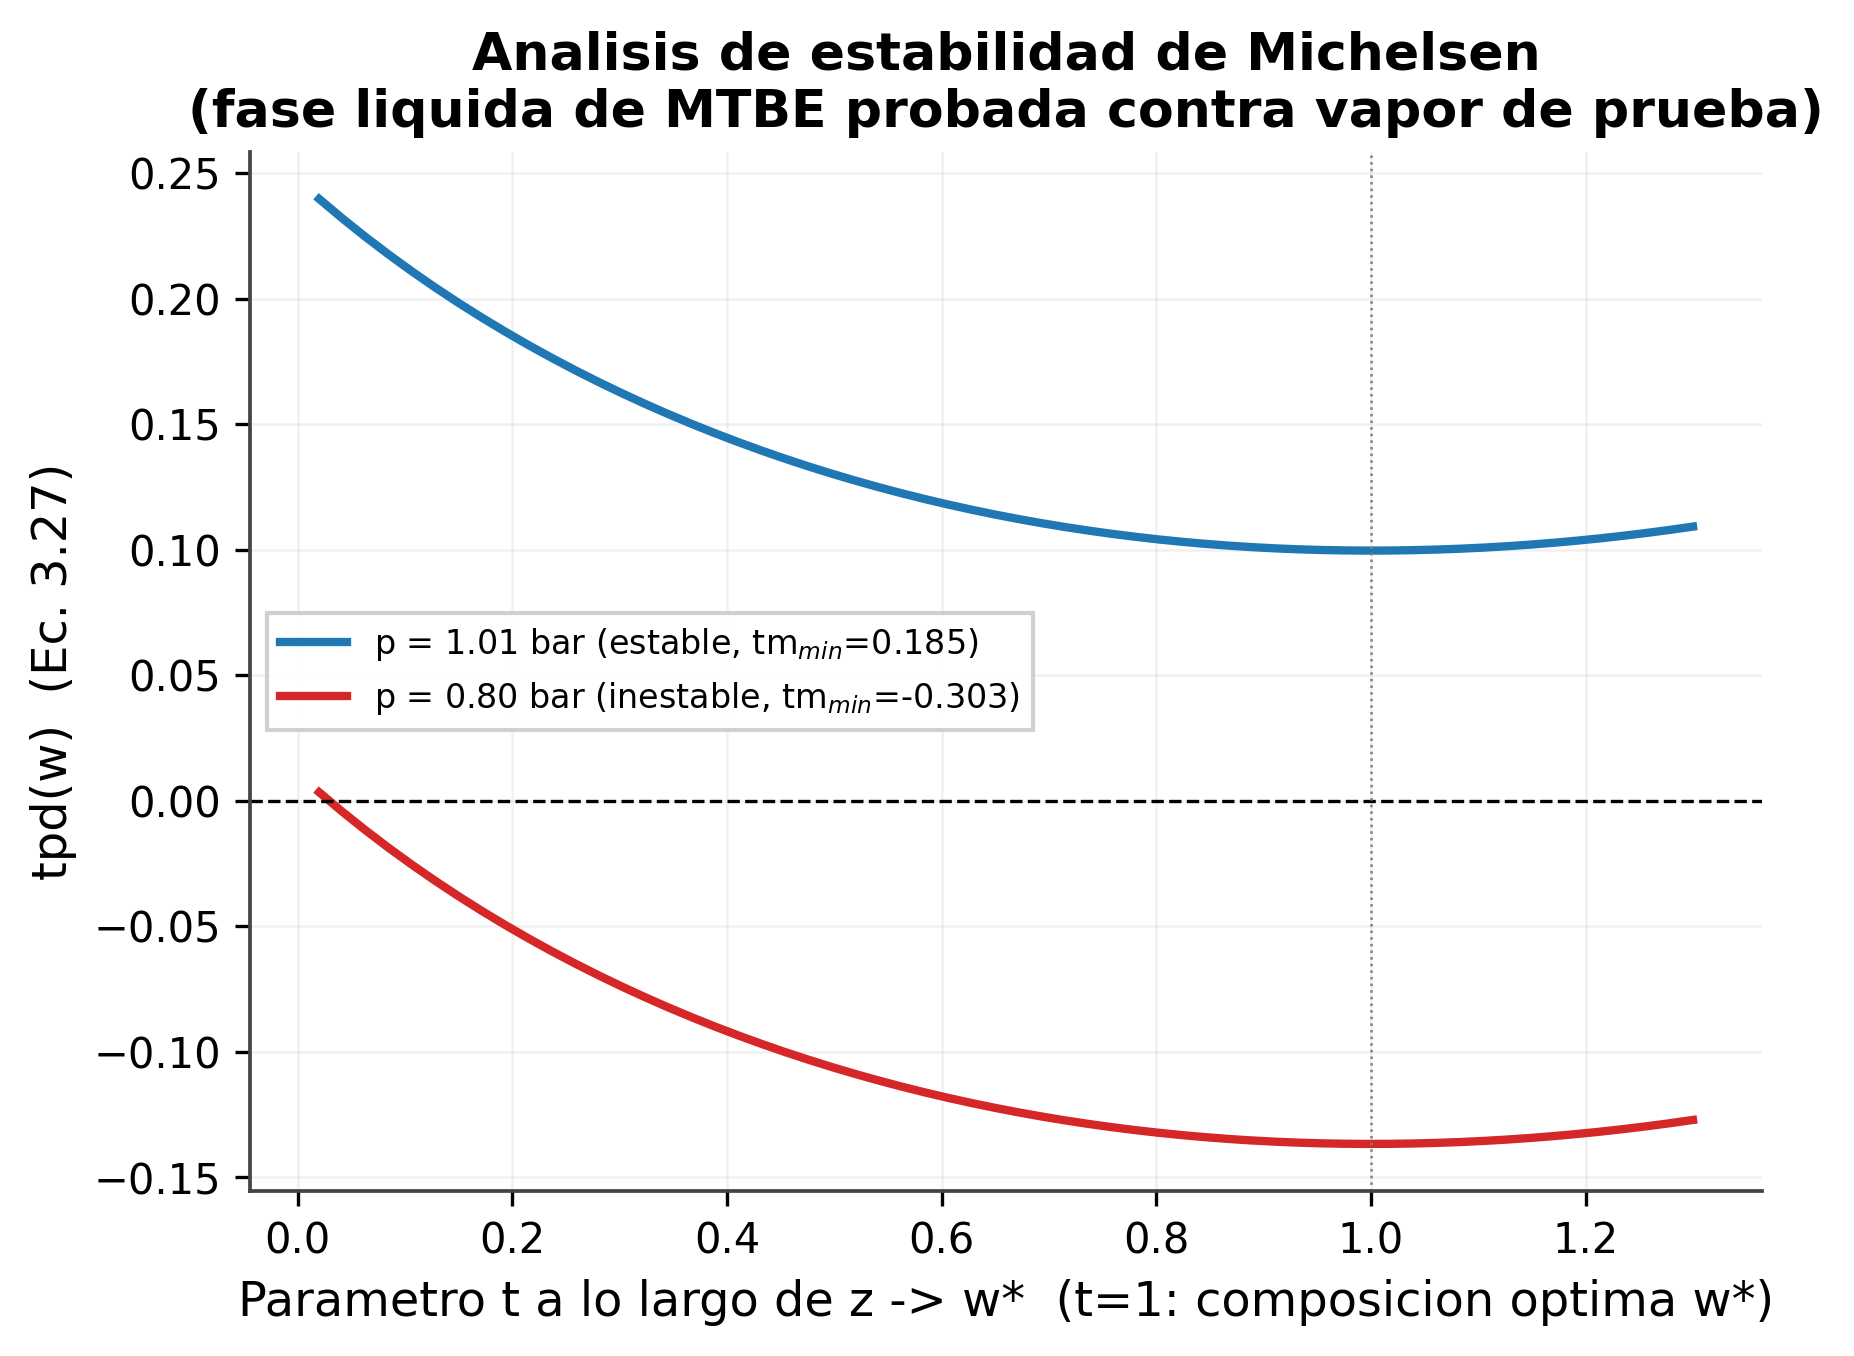
\includegraphics[width=0.78\textwidth]{figuras/estabilidad_tpd.png}
\caption{Función $\mathrm{tpd}(w)$ (Ec.~\eqref{eq:3.27}) para la fase
líquida de MTBE, probada contra una fase vapor de prueba, a dos
presiones: $p=1.01325$~bar (estable, $\mathrm{tpd}\geq 0$ en todo el
dominio) y $p=0.80$~bar (inestable, $\mathrm{tpd}<0$ para algunas
composiciones de prueba).}
\label{fig:tpd}
\end{figure}

\begin{figure}[h]
\centering
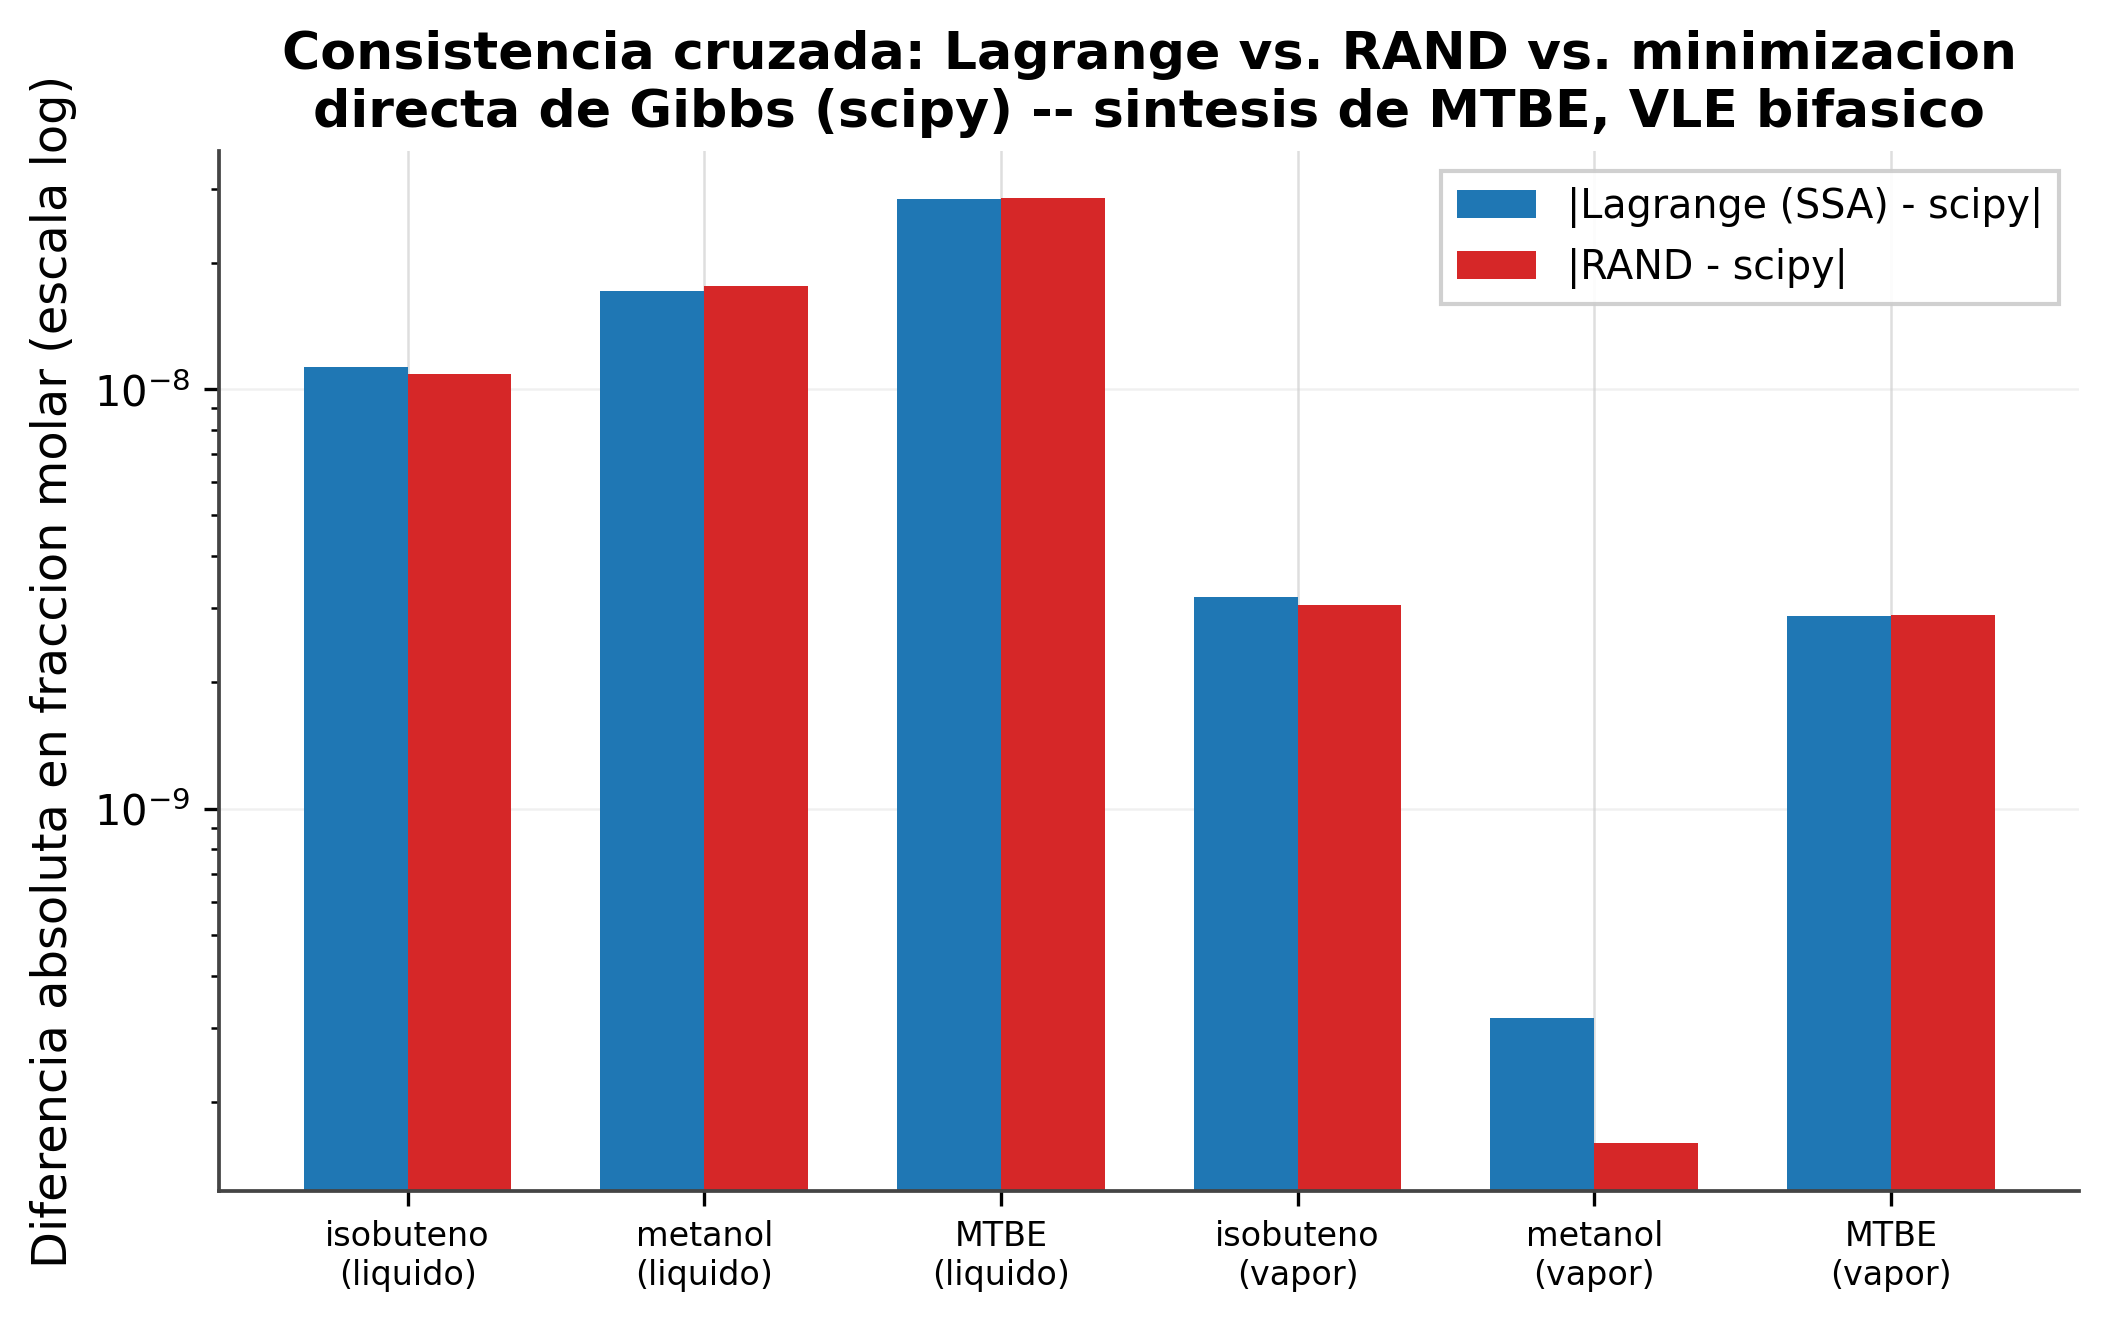
\includegraphics[width=0.85\textwidth]{figuras/comparacion_solvers.png}
\caption{Diferencia absoluta en fracción molar entre el método de
Lagrange (SSA), el RAND modificado, y una minimización directa de
Gibbs con \texttt{scipy.optimize} (referencia independiente), para el
sistema MTBE bifásico. Todas las diferencias están por debajo de
$10^{-6}$.}
\label{fig:comparacion-solvers}
\end{figure}

\begin{figure}[h]
\centering
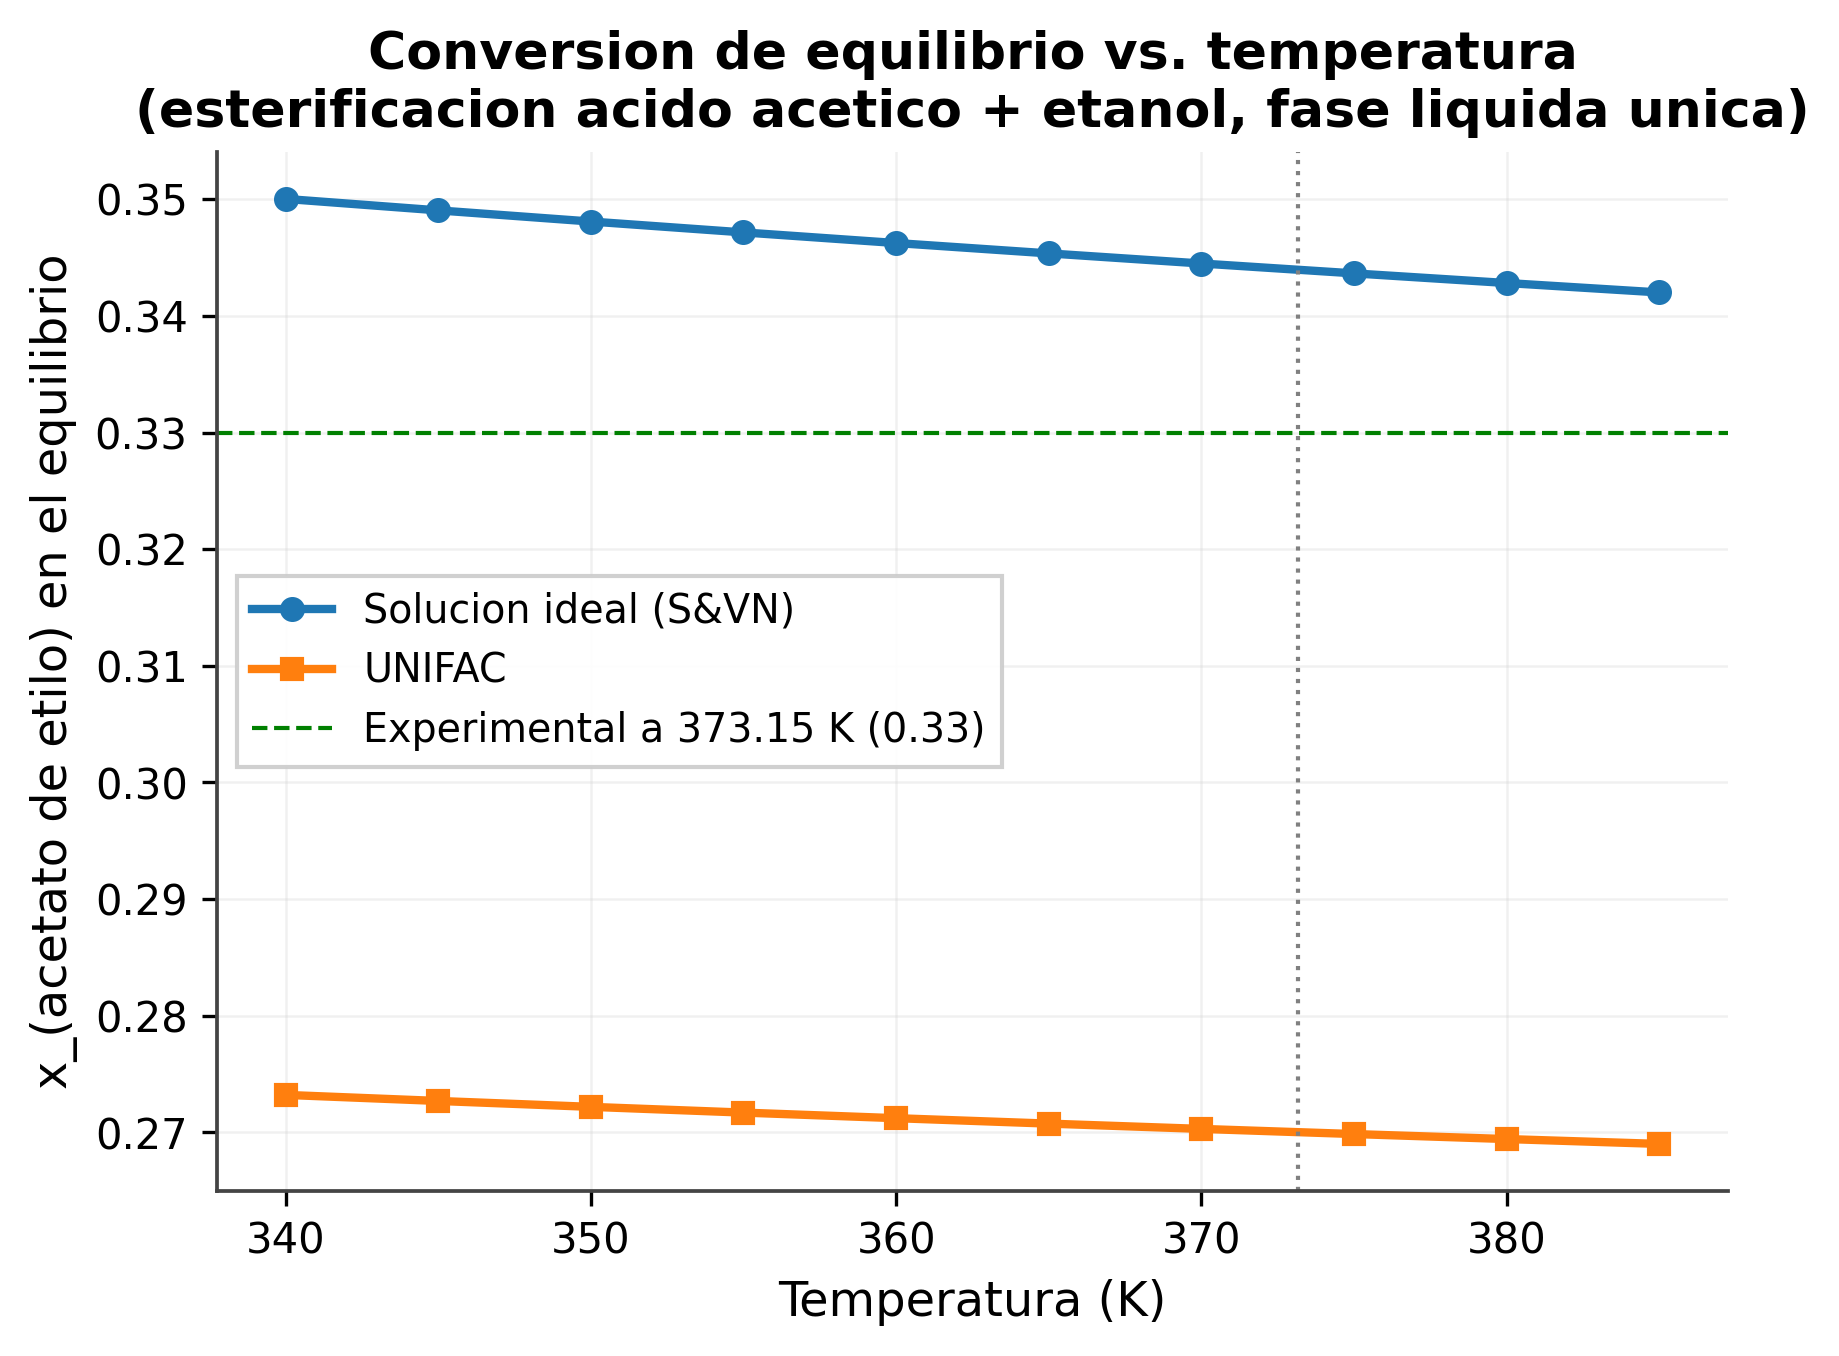
\includegraphics[width=0.75\textwidth]{figuras/acetic_etanol_conversion.png}
\caption{Conversión de equilibrio ($x_{\text{EtAc}}$) en función de la
temperatura, fase líquida única, para los modelos ideal y UNIFAC. La
línea verde marca el dato experimental citado por
\citet{smithvannessabbott} a 373.15~K.}
\label{fig:conversion-T}
\end{figure}

% =====================================================================
\section{Conclusiones}
\label{sec:conclusiones}
% =====================================================================

\subsection{Qué se validó}

\begin{itemize}
  \item Las ecuaciones 3.14--3.78 de \citet{tsanas2018} fueron
    reconstruidas directamente del texto del PDF original (no de una
    conversión a Markdown dañada) y verificadas internamente mediante
    diferencias finitas de Jacobianos y derivadas composicionales.
  \item El método RAND modificado reproduce el ejemplo numérico
    publicado por Greiner~\citep{greiner1991} con una diferencia de
    $\sim 8\times 10^{-6}$, incluyendo la reproducción del fracaso
    documentado del método de aproximación ideal en el mismo sistema.
  \item El método de Lagrange reproduce exactamente el Example 14.8 de
    \citet{smithvannessabbott}.
  \item Los tres métodos de solución (Lagrange, RAND, minimización
    directa con scipy) convergen al mismo resultado en todos los casos
    de prueba, con tolerancia $10^{-8}$ o mejor.
  \item Se extendió la validación a un sistema de VLE completo con
    reacción (esterificación a 355~K), usando datos de Antoine
    verificados de dos fuentes distintas y un modelo UNIFAC con grupos
    oficiales DDBST, obteniendo tendencias cualitativas consistentes
    con la Tabla 4.4 de la tesis.
\end{itemize}

\subsection{Limitaciones}
\label{sec:limitaciones}

\begin{itemize}
  \item \textbf{Parámetros de la tesis no disponibles.} Ninguno de los
    documentos disponibles para este proyecto (la tesis convertida a
    Markdown, el PDF original, ni los libros de texto consultados)
    contiene los parámetros de Wilson/UNIQUAC, Antoine, o $K_{\text{eq}}(T)$
    usados en los casos de estudio del Capítulo 4 de
    \citet{tsanas2018} (MTBE: \citet{ungdoherty1995}; esterificación:
    \citet{xiao1989}). Por lo tanto, ninguna de las Tablas 4.2, 4.4,
    4.6 u 4.8 de la tesis se reproduce numéricamente; la comparación
    con la Tabla~4.4 es cualitativa.
  \item \textbf{Gap de robustez en el arranque de fases.} El análisis
    de estabilidad (\texttt{estabilidad.py}) y la adición automática de
    fases (\texttt{algoritmos.py}) no son robustos para sistemas
    fuertemente no ideales cuando se arranca desde una sola fase (por
    ejemplo, UNIFAC en el sistema de esterificación). Este problema fue
    identificado explícitamente y \textbf{no se resolvió} en este
    trabajo, por decisión explícita de alcance; los casos de validación
    que lo habrían disparado se resolvieron fijando el número de fases
    de antemano.
  \item \textbf{No se implementaron ecuaciones de estado reales}
    (Peng-Robinson, SRK, etc.); todas las fases vapor se modelaron como
    gas ideal.
\end{itemize}

\subsection{Trabajo futuro}

\begin{itemize}
  \item Resolver el gap de robustez del arranque de fases, posiblemente
    mediante regularización adicional de la matriz $M_k$ para
    componentes en trazas o eliminación dinámica de fases que colapsan
    a cantidad cero.
  \item Si se consiguen los parámetros originales de
    \citet{ungdoherty1995} o \citet{xiao1989}, repetir la validación
    numérica directa contra las Tablas 4.2--4.8 de la tesis.
  \item Extender \texttt{termodinamica.py} con una ecuación de estado
    cúbica real (Peng-Robinson) para sistemas con fase vapor no ideal,
    como el de síntesis de amoníaco estudiado por
    Binous y Bellagi.
\end{itemize}

% =====================================================================
\bibliographystyle{plainnat}
\bibliography{referencias}

\end{document}
